We conclude this report by a short appendix dedicated to providing some details about the concrete implementation of the methods we discussed throughout this report.
We start by giving some informal ideas about where the computational cost of a molecular simulation is concentrated, before discussing the process of choosing a software to implement various non-equilibrium methods.
We finally give a short summary of the implementations we made, pointing the reader to the relevant sources.

\section{Scaling of the computational cost}
Throughout this document, the reader will notice that little is said about $\nabla V$, meaning the methods we described simply invoked $\nabla V$ where it is needed, 
without getting into the specifics of \textit{how} it is computed.
For a pair interaction potential of the form \eqref{eq:lennard_jones}, the naive method of summing over all pairs of particles incurs a cost of
\[\frac{N(N-1)}2 =\mathrm{O}(N^2)\]
evaluations of the pair interaction function $v$.
Another point we alluded to is that the statistical error on the computation of averages usually dissipates at a rate $\mathrm{O}(1/\sqrt{\Dt N_{\mathrm{iter}}})$.
Furthermore, for averages to be physically meaningful, $N$ must be taken large enough for the thermodynamic limit to be considered reached.
In practice, a quadratic scaling of the computational cost of computing $\nabla V$ may render essentially impossible the computation of long numerical trajectories.
Instead, one has to rely on approximate evaluations of $\nabla V$. For instance, in the case of a Lennard-Jones interaction, the pair interaction potential decays quickly, in $\mathrm{O}(r^{-6})$ as a function of the interparticular distance $r$.
In this case, a reasonable approximation consists on imposing a fixed maximal interaction distance $r_c$, called the \textit{cutoff} distance, and asserting that particles which are further apart that $r_c$ do not interact.
This amounts mathematically to replacing the pair interaction function $v(r)$ by a cut-off version $v(r)\1_{r<r_c}$, effectively modifying the potential.
There are various ways to alter this procedure in order to make the modified potential continuous or $C^1$, for instance using spline interpolation. 
Of course, this procedure alone does not solve anything, since one still needs to determine \textit{which} pairs of particles are neighbors, meaning they are closer apart than $r_c$, which still amounts to $\mathrm{O}(N^2)$ computations of the (squared) Euclidean norm.
To make this viable, one has to store a list of neighbor pairs in an efficient data structure which only needs to be updated once every few simulation iterations, since the set of neighboring pairs tend not to drastically change over short time intervals.
In practice, and depending on the timestep, the meaning of the word \textit{few} can sometimes be understood to be as large as $50$.
There are various strategies to implement such a data structure, such as Verlet lists or cell lists, which are described in detail in \cite[Section 5.3]{AT89}.
At any rate, since the number of neighbors to a given particle should on average be close to $4\pi\rho r_c^3/3=\mathrm{O}(1)$, where $\rho$ is the particle density, the cost of computing $\nabla V$ becomes (ideally) \textbf{linear} in $N$,
which makes long time simulations a practical possibility. 
We mention the issue of short-range interactions since all our molecular simulations used $V$ of the Lennard-Jones form, but other methods exist in the case where $V$ decays slowly like the Coulomb electrostatic potential, relying in this case on a fast decay property in Fourier space.
Of course, many more tricks exists, which collectively form the whole craftsmanship of Molecular Dynamics (MD) simulations: finding efficient, approximate ways to compute $V$ and $\nabla V$.

\section{Selecting a Molecular Dynamics package}
The process of implementing from scratch these methods is time consuming, and unnecessary given the number of freely available MD packages. 
However, some of these packages are quite ancient and heavily optimized so that the process of implementing new methods comes with quite a heavy learning overhead, as well as being harder to debug.
Instead, we chose to make use of a Julia package for MD simulation, thus taking this opportunity to learn the programming language Julia \cite{bezanson2017julia}, which has been gaining a lot of traction in the scientific computing user base, 
in part because it offers the shared benefit of performance comparable to that of C or C++, as well as possessing a rich ecosystem of highly intercompatible packages, powered by a strong community and a design philosophy centered around generic, type-agnostic, interfaces.

The first step in the internship consisted in choosing a package between two contenders, NBodySimulator \cite{NBS}, and Molly \cite{Molly}. 
NBodySimulator, in summary, acts as a wrapper around the native differential equations Julia framework, constructing a differential equation or stochastic differential equation from the specification of a molecular system.
As such, it aims to compute \textit{exact} solutions to the dynamics, or at least exact evaluations of $V$. 
On the other hand, Molly offers a number of neighbor-finding strategies, such as the cell list method, a parallelized naive iteration over all pairs of neighbors, as well as a tree-search based method. 
In Figure \ref{fig:linear_scaling}, we show the results of a comparison of the scaling of the simulation time as a function of the system size, for NBodySimulator and Molly's various neighbor finding strategies.
We find that, if for very small systems, NBodySimulator outperforms Molly, the advantage quickly disappears, for $N \geq 750$ approximately, in the case of the cell list method.
Interestingly, even the naive double loop for Molly overtakes NBodySimulator in performance. This is because by default, Molly parallelizes the force computation, while there is no parallelization in NBodySimulator.

\begin{figure}[htbp]
    \begin{center}
      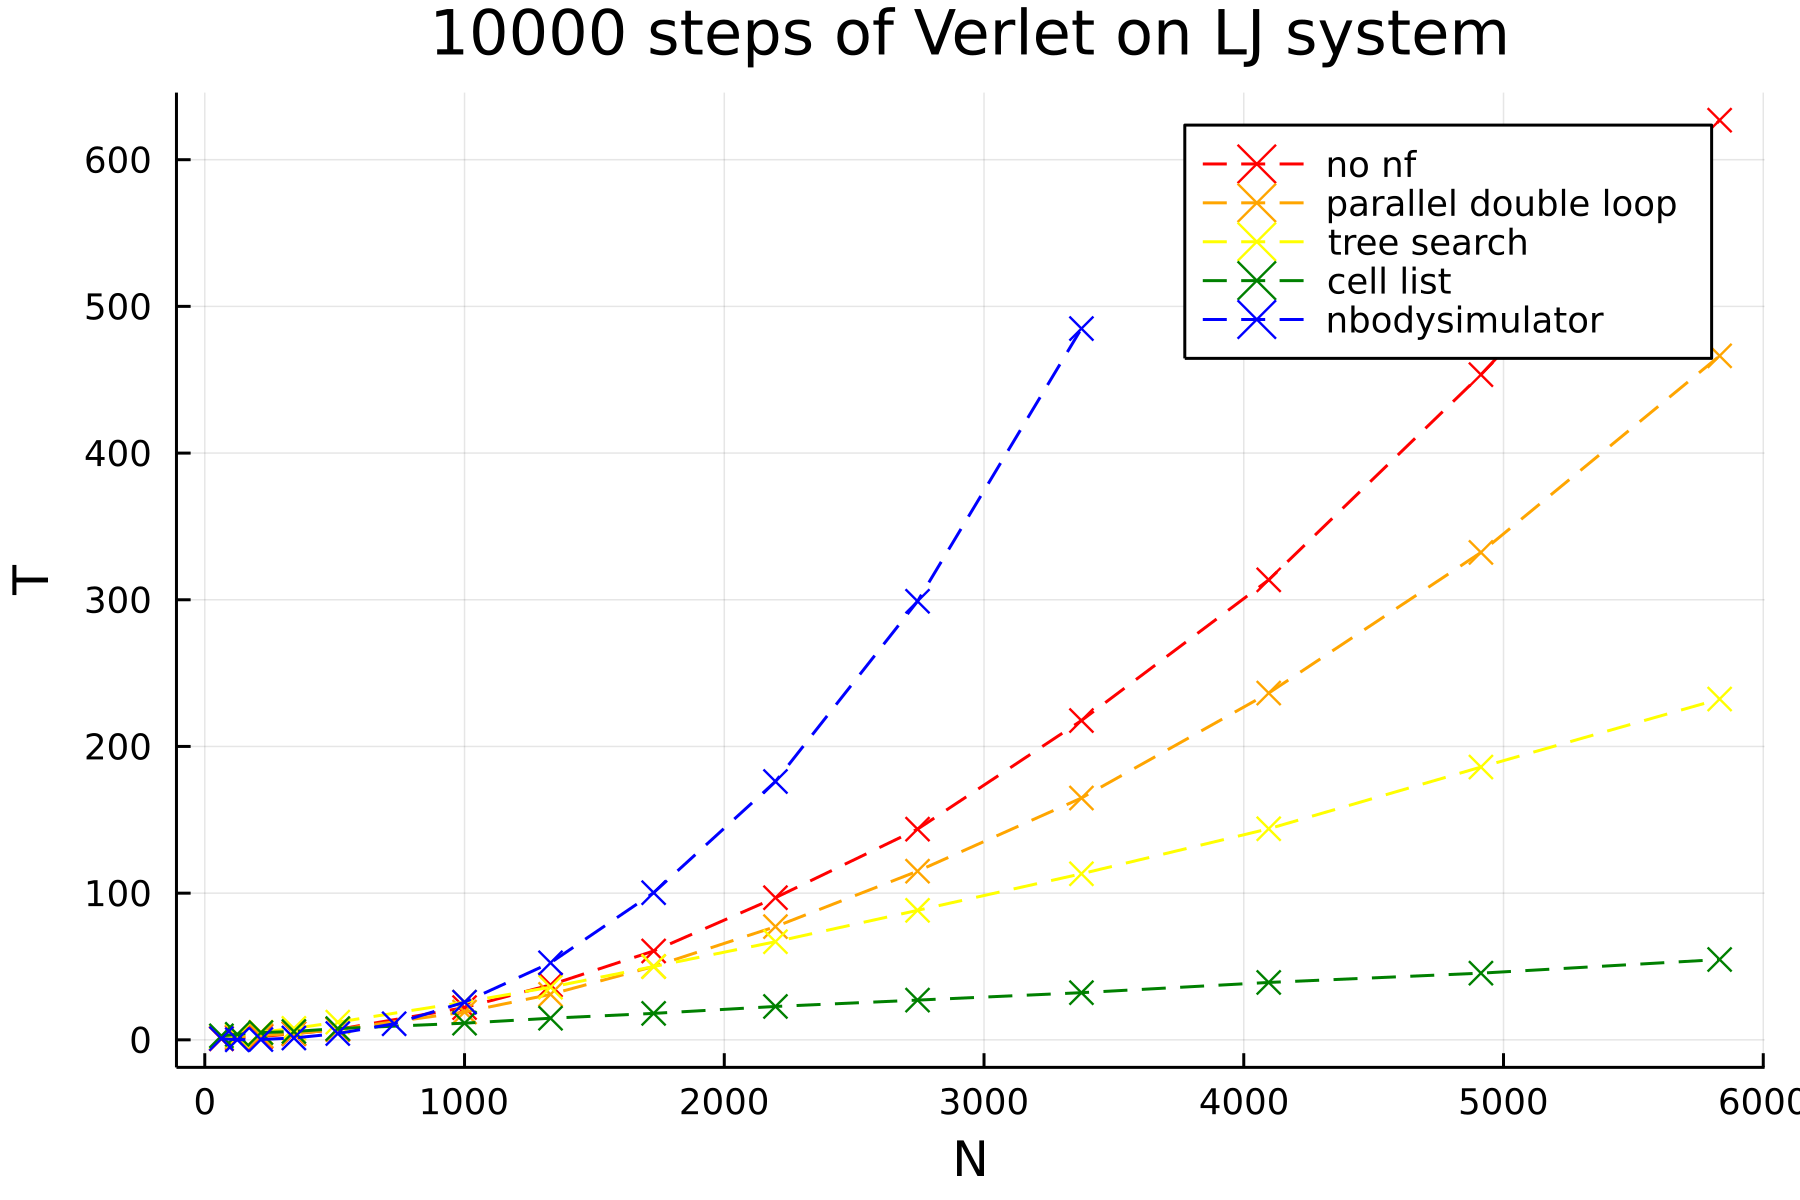
\includegraphics[width=0.7\linewidth]{figures/appendix/scaling_comparison_full.png}
      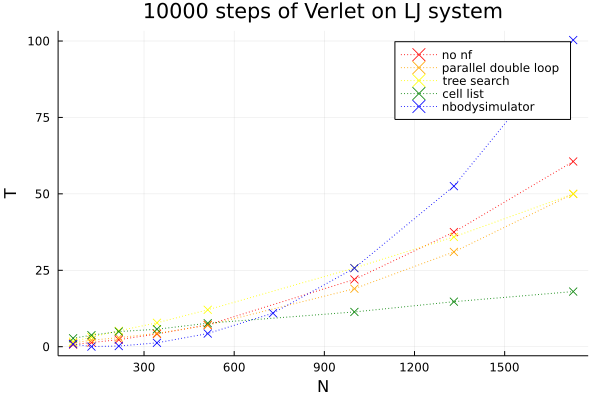
\includegraphics[width=0.7\linewidth]{figures/appendix/scaling_smallN.png}
      \caption{ \label{fig:linear_scaling}
        Comparison of world clock time for the simulation of 10000 steps of a Lennard-Jones system. The "no nf" corresponds to the naive double loop. Top: full curve. Bottom: zoom on the small system regime.
      }
    \end{center}
  \end{figure}

On this basis, we chose to implement our methods in Molly.

\section{Summary of implementations}
Along the way, some of our implementations were integrated in the Molly source, in large part during a one-week stay in the MRC Laboratory of Molecular Biology in Cambridge, where the main author of Molly's source code, Joe Greener, works.
These integrations include:
\begin{enumerate}[i)]
    \item A cutoff strategy based on a cubic spline interpolation,
    \item A general Langevin integrators, which works for all splitting orderings \eqref{eq:splitting_ordering} and in the (non)-equilibrium setting,
    \item A logger to efficiently estimate time correlations functions of the form \eqref{eq:time_correlation},
    \item A logger to track the self-diffusion coordinates \eqref{eq:self_diffusion_process} for Einstein mobility computations,
    \item A refactoring of Molly's general logging architecture, for more flexibility and extensibility,
    \item The addition of a parameter for Boltzmann's constant, allowing for fully consistent sets of user-defined custom systems of units,
    \item An online ergodic average and asymptotic variance estimator for a user-specified observable.
\end{enumerate}
These were additionally documented, and non-regression tests were implemented for each of them. We refer the reader to the Molly documentation and source code for more details.
Other implementations were too use-specific, not general or not mature enough to be integrated. These include
\begin{enumerate}[i)]
    \item A pressure observable based on \eqref{eq:pressure},
    \item The implementation of NEMD force fields for mobility and shear viscosity computations,
    \item The implementation of an integrator for the Norton method,
    \item Various logging and visualization utilities.
\end{enumerate}
These implementations are available in the repository \cite{myrepo}, although we apologize in advance to the interested reader for the poorly organized, largely uncommented mess that lies within.
We expect, especially for the pressure observable, that a future integration in Molly will be possible, for instance once long-range force contributions are implemented, as well as a more flexible interface for force computations.
This will be a necessary step in the implementation of barostats, which are important in the context of biomolecular simulation, a use case Molly is particularly attuned to.
On the other hand, non-equilibrium methods are unlikely to have a place in a general-purpose MD package.
Instead, we might consider publishing in the future a standalone package that extends Molly for transport coefficient computations, once our understanding of the Norton method has cohered.